

\documentclass{beamer}

\usepackage[T1]{fontenc}
\usepackage[utf8]{inputenc}
\usepackage[french,english]{babel}

\usepackage{lmodern}
\usepackage{amsthm}
\usepackage{float}
\usepackage{lmodern}%pour un meilleur rendu des polices
\usepackage{verbatim}%du texte non interprt
\usepackage{amsmath}
\usepackage{amssymb}%maths
\usepackage{xspace}
\usepackage[dvipsnames,svgnames,table]{xcolor}
\usepackage{listings}
\usepackage{fancyhdr}
\usepackage{etoolbox}
\usepackage{titlesec}
\usepackage{titletoc}
\usepackage{lastpage}
\usepackage{hyperref}
\usepackage{ctable} % for \specialrule command
\usepackage{cite}
\usepackage{algorithm2e}
\usepackage{alltt}
\usepackage{array}
\usepackage{mdwmath}
\usepackage{mdwtab}
\usepackage{eqparbox}
\usepackage{subfig}
\usepackage{dblfloatfix}
\usepackage{url}
\usepackage{tipa}
\usepackage{stmaryrd}
\usepackage{upgreek}
\usepackage{mathrsfs}
\usepackage{ulem}
\usepackage{cancel}

\graphicspath{{img/}}
\DeclareGraphicsExtensions{.pdf,.jpeg,.jpg,.png}


\newcommand{\ccite}[1]{\textbf{\cite{#1}}}
\newcommand{\pd}[2]{\dfrac{\partial #1}{\partial #2}}
\newcommand{\od}[2]{\dfrac{\mathscr{D}_a #1}{\mathscr{D} #2}}
\newcommand{\tensor}[1]{\mathbf{#1}}
\renewcommand{\vector}[1]{\overrightarrow{#1}}

\newcommand{\Tau}{\tensor{\mathlarger{\uptau}}}
\renewcommand{\v}{\vector{u}}
\newcommand{\W}{\tensor{W\left( \v \right)}}
\newcommand{\D}{\tensor{D\left( \v \right)}}
\newcommand{\grad}{\vector{\nabla}}
\newcommand{\gradv}{\tensor{\nabla\v}}
\renewcommand{\div}[1]{div \left( #1 \right)}
\newcommand{\divv}[1]{\vector{div} \left( #1 \right)}
\newcommand{\UU}{\mathcal{U}}
\newcommand{\VV}{\mathcal{U}}
\newcommand{\M}{\mathcal{M}}
\newcommand{\A}[2]{\mathcal{A}_{#1}\left( #2 \right)}
\newcommand{\Uu}{\UU^{n}}
\newcommand{\Uv}{\UU^{n+\theta}}
\newcommand{\Uw}{\UU^{n+1-\theta}}
\newcommand{\Ux}{\UU^{n+1}}
\newcommand{\Uk}{\UU^{k}}
\newcommand{\Ukk}{\UU^{k+1}}
\newcommand{\Vk}{\VV^{k}}
\newcommand{\Vkk}{\VV^{k+1}}
\newcommand{\Tauk}{\Tau^{k+1}}
\newcommand{\vk}{\v^{k+1}}
\newcommand{\pk}{p^{k+1}}
\newcommand{\Dk}{\tensor{D\left( \vk \right)}}

\definecolor{lightgray}{gray}{0.9}
\definecolor{titlecolor}{RGB}{0,0,200}
\definecolor{subtitlecolor}{RGB}{0,0,153}
\definecolor{textcolor}{RGB}{0,128,255}
\definecolor{RoyalPurple}{RGB}{102,51,153}
\definecolor{ForestGreen}{RGB}{34,139,34}


\newcommand{\colbox}[1]{\colorbox{lightgray}{$ #1 $}}

\newcommand{\stitle}[2][0.3cm] { 
    {\normalsize \textcolor{titlecolor}{\textbf{#2}}} 
    \vspace{#1} 
}

\newcommand{\ssubtitle}[1]{ {\footnotesize \textcolor{subtitlecolor}{\textbf{#1}}} }

\newcommand{\stress}[1]{\textcolor{textcolor}{#1}}

\newcommand{\hidecontent}[2][0.25]{{% \hidecontent[<transparency>]{<stuff>}
  \setbox9=\hbox{#2}% Store <stuff> in \box9 to obtain height/width
  \transparent{#1}\ooalign{\usebox9\cr\color{white}\rule{\wd9}{\ht9}\cr}}}



\usetheme{Frankfurt}
\def\beamertemplatetransparentcoveredmedium{\setbeamercovered{transparent=40}}
\def\beamertemplatetransparentcoveredhard{\setbeamercovered{transparent=20}}
\beamertemplatetransparentcoveredmedium
\setbeamertemplate{bibliography item}[triangle]
\addtobeamertemplate{footline}{\hfill\insertframenumber/\inserttotalframenumber\hspace{2em}\null}

\begin{document}


\title{\Large Scattered Data Interpolation using Wavelet Trees}
\author[Keck]{\Large Jean-Baptiste Keck}
\institute[MSIAM]{\Large \bsc{M2 Msiam}}
\date{\large Paper Review\\ 10/02/2015}


\begin{frame}
    \titlepage
\end{frame}


\begin{frame}{Interpolating wavelets} 
    \stitle{Building interpolation wavelets}
    \footnotesize

    \begin{itemize}
        \item Classical interpolation tools can be fitted into a MRA framework.
    \end{itemize}

    \begin{block}{Interpolating scaling function}
        $\P$ is an interpolating scaling function 
        $
        \Leftrightarrow
        \left\{
        \begin{array}{l c l l}
            \P(0) & = & 1 & \\
            \P(k) & = & 0 & \forall\ k \in \Z^* \\
        \end{array}
        $
    \end{block}
    
    \begin{itemize}
        \item Built as infinite convolution of discrete filters
            $\Ph(\nu) = \prod_{k=1}^{+\infty} m_0(\frac{\nu}{2\pi})$ 
        \vskip 0.3cm
        \item Interpolating property can be expressed as $m_0(\nu) + m_0(\nu + \pi) = 1$
        \vskip 0.3cm
        \item $\P$ has compact support $\Leftrightarrow h_n$ is finite $\Rightarrow$ Approximation order is finite 
        \vskip 0.3cm
        \item \textbf{Families :} Splines functions, \alert{Deslauriers-Dubuc interpolating wavelets}
    \end{itemize}
\end{frame}

\begin{frame}{Deslauriers-Dubuc interpolating wavelets} 
    \ssubtitle{Lagrange interpolation :}
    \footnotesize
    
    \begin{itemize}
        \item Can explicitely compute filter coefficients \alert{$h_n$} with Lagrange polynomials of order $\alert{p}\ \forall n \in \llbracket -2p+1, 2p-1 \rrbracket$.
    \end{itemize}
  
    \vskip 0.2cm
    \ssubtitle{Dyadic refinement scheme :}
    \vskip -0.3cm
    \begin{figure}[H]
        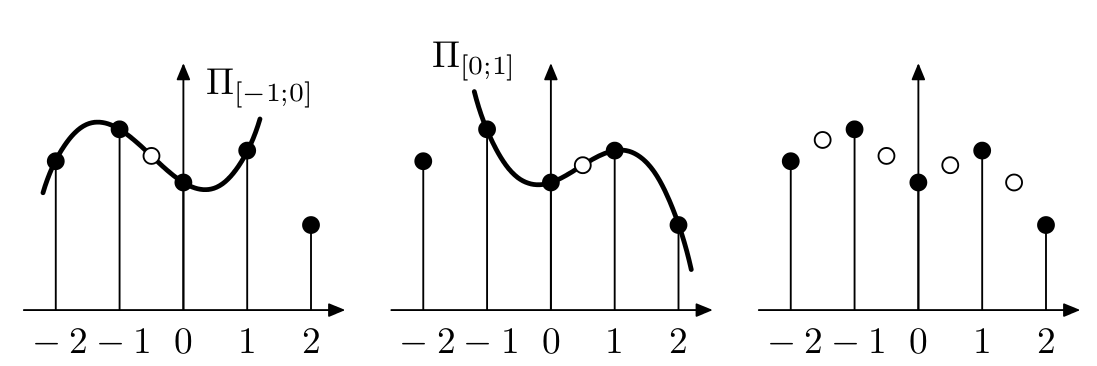
\includegraphics[scale=0.2]{lagrange}
    \end{figure}

    \begin{block}{Low pass filter coefficients $h_n$}
    $
    \begin{array}{l cc c cc r}
        m_0[0] = 1 && 
        m_0[2k] = 0 \textrm { if } k \in \Z^* &&
        m_0[k] = 0 \textrm{ if } |k| \geq 2p& \\
        \\
        \multicolumn{7}{l}{
            m_0[\pm (2k-1)] = \dfrac{(-1)^{k+1}(2p)!^2}{2^{4p}p!^2(p-k)!(p+k-1)!(2k-1)}\ \ \ \forall k \leq p
    }
    \end{array}
    $
    \end{block}
\end{frame}

\begin{frame}{Generation of the scaling function} 
    
    \footnotesize
    
    \ssubtitle{Generate $\P_p$ at resolution $2^{-j}$ with j convolutions $\delta_{x,0} \ast h_n^p \ast \cdots \ast h_n^p$ :}
   
    \only<1>{
        \begin{figure}[H]
            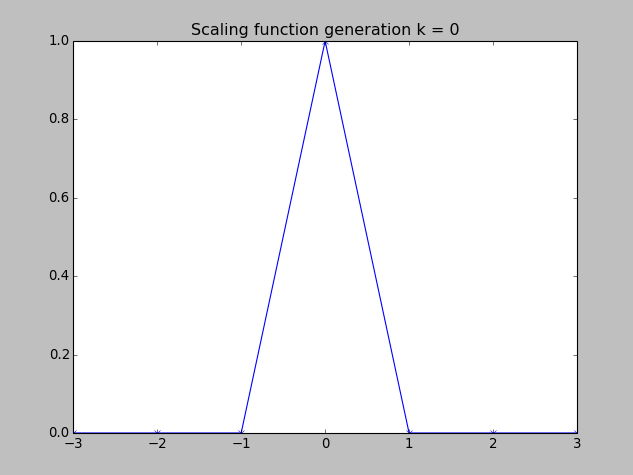
\includegraphics[scale=0.4]{scaling_10}
        \end{figure}
    }
    \only<2>{
        \begin{figure}[H]
            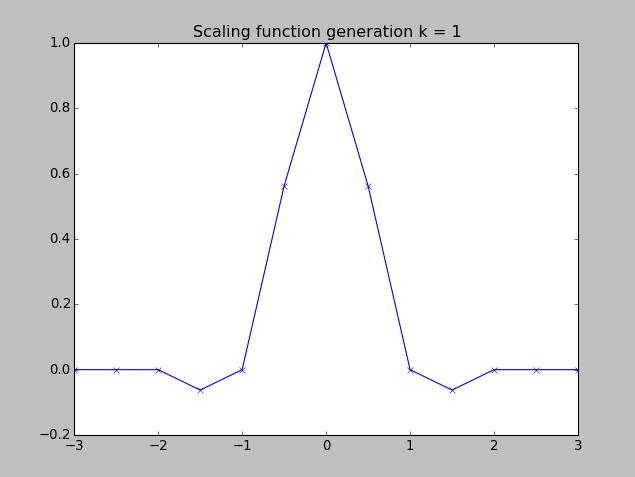
\includegraphics[scale=0.4]{scaling_11}
        \end{figure}
    }
    \only<3>{
        \begin{figure}[H]
            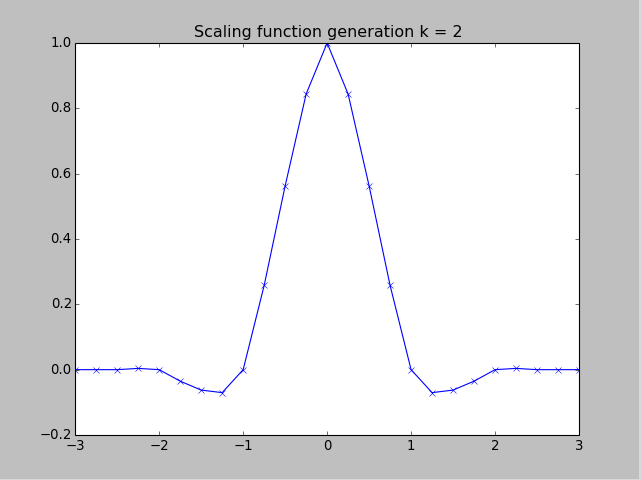
\includegraphics[scale=0.4]{scaling_12}
        \end{figure}
    }
    \only<4>{
        \begin{figure}[H]
            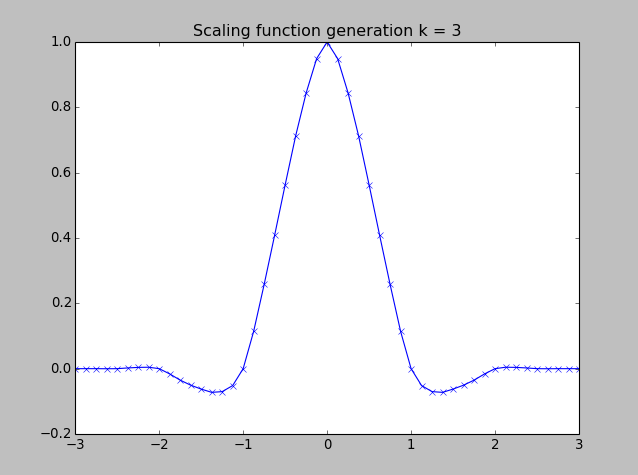
\includegraphics[scale=0.4]{scaling_13}
        \end{figure}
    }
    \only<5>{
        \begin{figure}[H]
            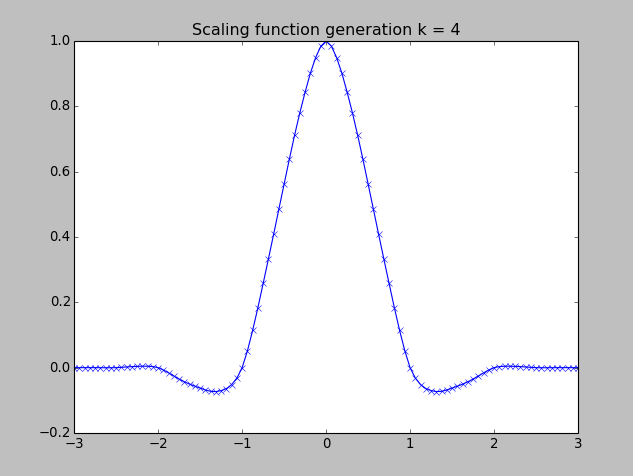
\includegraphics[scale=0.4]{scaling_14}
        \end{figure}
    }
    \only<6>{
        \begin{figure}[H]
            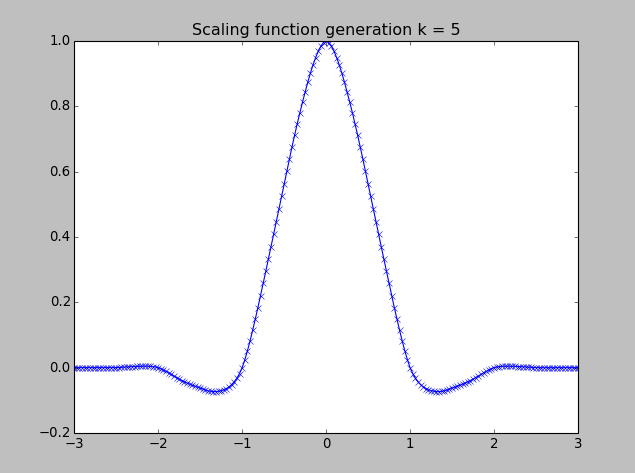
\includegraphics[scale=0.4]{scaling_15}
        \end{figure}
    }
\end{frame}
    

\begin{frame}{Properties} 

    \ssubtitle{Basis definition in the dyadic case:}
    \begin{itemize}
        \item  Scaling function : $\P$(x) is of order p
        \item  Mother wavelet : $\Psi(x) = \P(2x - 1)$
        \item  Wavelet family : $\Psi_{jk} = \Psi(2^j x - k)$
        \item  Basis : $\mathcal{B}_0 = \{ \Psi_{jk}\ |\ \underbrace{j = 0}_{V_0} \textrm{ \alert{or} } \underbrace{(j,k) \in \N^* \times (2\Z + 1)}_{W_{j-1}} \}$
    \end{itemize}

    \ssubtitle{Properties :}
    
    \begin{itemize}
        \item Symmetry
        \item Finite support $\subset [-2p+\frac{1}{2}, 2p-\frac{1}{2} ]$
        \item \alert{No orthogonality} $\Rightarrow$ need to solve a linear system
        \item $2p$ vanishing moments
    \end{itemize}
    
    \ssubtitle{Wavelets on the interval (boundary problems) :}
    \begin{itemize}
        \item Take \alert{boundary filters of lower order}
    \end{itemize}
    
\end{frame}

\begin{frame}{Wavelets on the interval : case $\Omega = [0,1]$ } 
    
    \ssubtitle{Boundary filters : Lowest resolution => Highest resolution}
    
    \only<1>{
        \begin{center}
            $V_0$
        \end{center}
        \vskip -0.3cm
        \begin{figure}[H]
            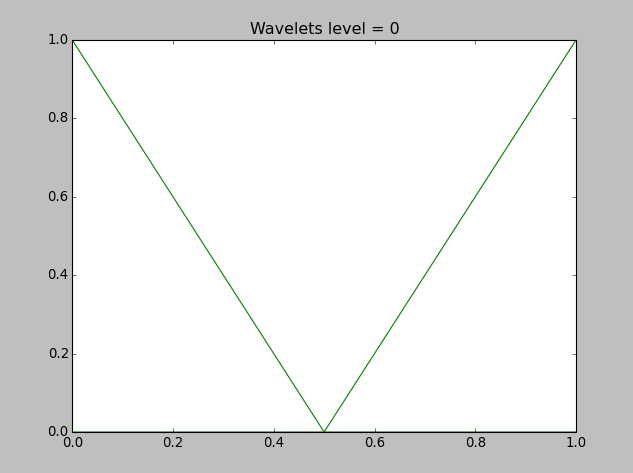
\includegraphics[scale=0.4]{interval_0}
        \end{figure}
    }
    \only<2>{
        \begin{center}
            $W_0$
        \end{center}
        \vskip -0.3cm
        \begin{figure}[H]
            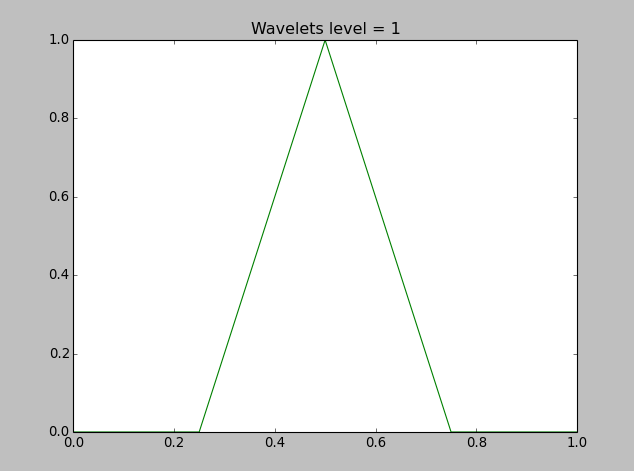
\includegraphics[scale=0.4]{interval_1}
        \end{figure}
    }
    \only<3>{
        \begin{center}
            $W_1$
        \end{center}
        \vskip -0.3cm
        \begin{figure}[H]
            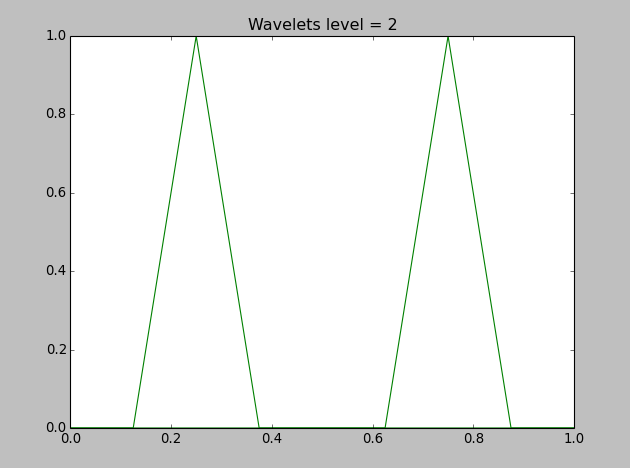
\includegraphics[scale=0.4]{interval_2}
        \end{figure}
    }
    \only<4>{
        \begin{center}
            $W_2$
        \end{center}
        \vskip -0.3cm
        \begin{figure}[H]
            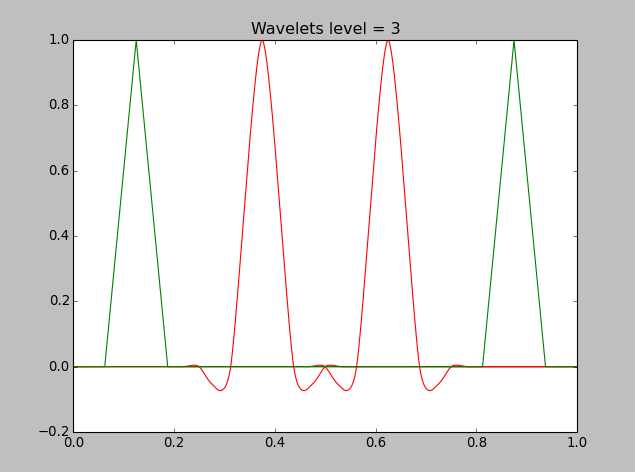
\includegraphics[scale=0.4]{interval_3}
        \end{figure}
    }
    \only<5>{
        \begin{center}
            $W_3$
        \end{center}
        \vskip -0.3cm
        \begin{figure}[H]
            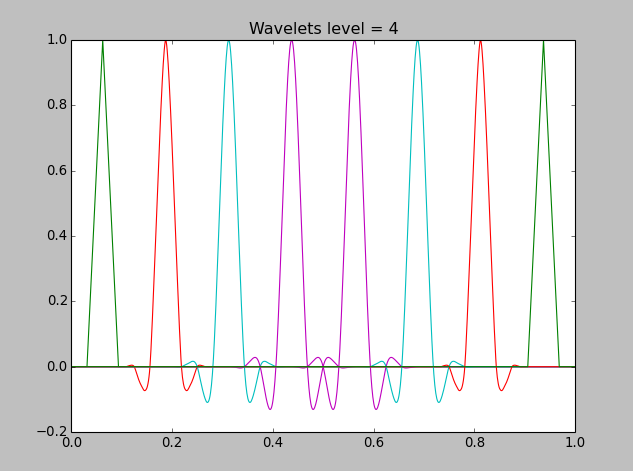
\includegraphics[scale=0.4]{interval_4}
        \end{figure}
    }
    \only<6>{
        \begin{center}
            $W_4$
        \end{center}
        \vskip -0.3cm
        \begin{figure}[H]
            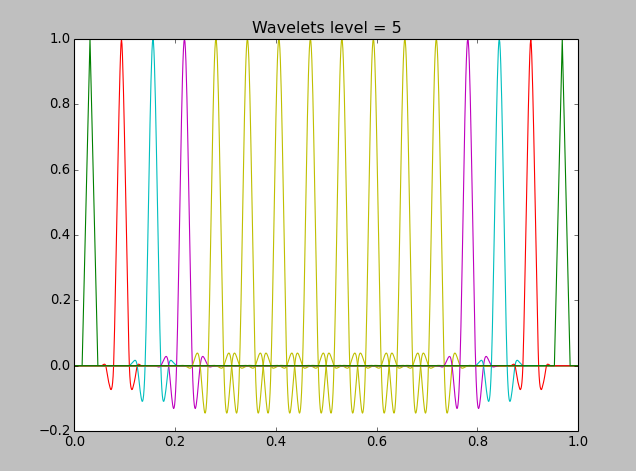
\includegraphics[scale=0.4]{interval_5}
        \end{figure}
    }

\end{frame}

\begin{frame}{Approximation in wavelet bases} 
    
    \stitle{Different approximations possible in wavelet bases :}
    \footnotesize

    \begin{itemize}
        \item \textbf{Exact wavelet decomposition :}
            {\scriptsize 
            $f = 
            \displaystyle \sum_{j=0}^{\infty} \displaystyle \sum_{k\in\Z} \langle f \mid \Psi_{jk} \rangle \Psi_{jk}
            = \displaystyle \sum_{j=0}^{\infty} \displaystyle \sum_{k\in\Z} \alert{d_{jk}} \Psi_{jk}$}

        \item \textbf{Linear approximation $\A_{lin}^{\alpha}$:} 
            $f \simeq \displaystyle \sum_{j=0}^{\alert{J}} \displaystyle \sum_{k\in\Z} d_{jk} \Psi_{jk}$
       
        \vskip 0.3cm
        \item \textbf{Non-linear approximation} $\A^{\alpha}$ (best N-terms approximation) : 
            $
            \abs{d_{j_0,k_0}} \geq
            \abs{d_{j_1,k_1}} \geq
            \cdots \geq
            \abs{d_{j_{N-1},k_{N-1}}}
            \Rightarrow
            f \simeq \displaystyle \sum_{i=0}^{\alert{N}} 
            d_{j_i,k_i}
            \ \psi_{j_i,k_i}
            $
        
        \vskip 0.1cm
        \item \stress{\textbf{Tree approximation}} $\T^{\alpha}$ :  Build a wavelet tree with following relationship
        \vskip 0.1cm
        \begin{center}
            $
            (j,k)\ \R\ (j',k') 
            \Leftrightarrow
            \left\{
            \begin{array}{l c l}
                j' & = & j + 1 \\
                k' & \in & \{2k - 1, 2k + 1\} \\
            \end{array}
            $
        \end{center} 

            \alert{Tree approximation spaces are close to non-linear spaces} (because singularities are located).
    \end{itemize}

\end{frame}

\begin{frame}{Example of wavelet tree structure} 
        \begin{figure}[H]
            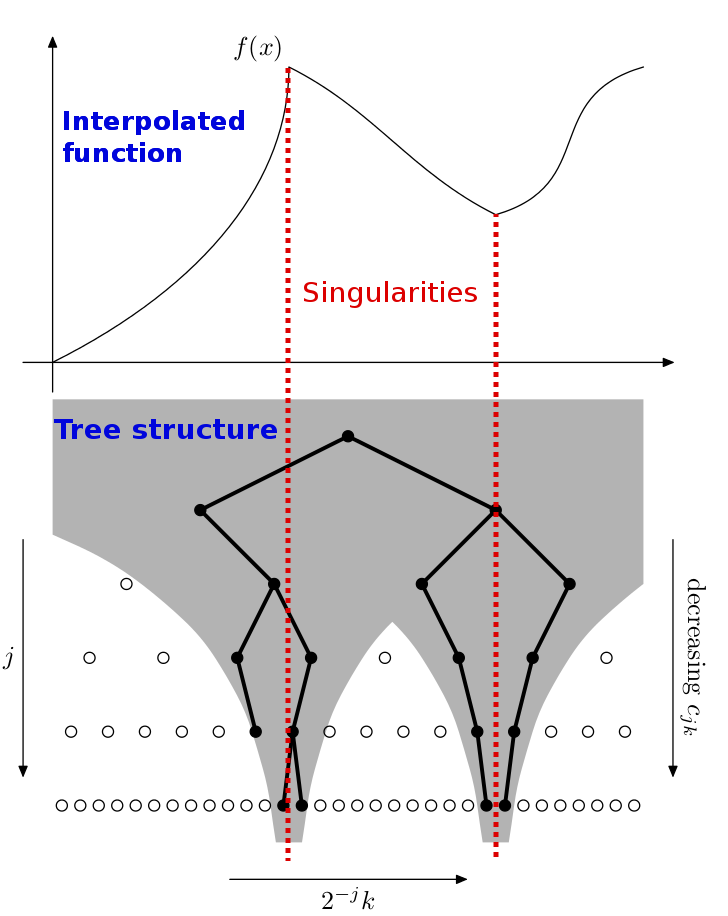
\includegraphics[scale=0.23]{tree_example}
        \end{figure}
\end{frame}

\begin{frame}{Scattered data interpolation}
    \stitle{Scattered data interpolation with wavelet trees:}
    \footnotesize
    \begin{itemize}
        \item \textbf{Input:} Set of \alert{N samples $\X \subset \mathbb{R}$} with corresponding sample values $\alert{f_{\X}} = \{ f(x) \ | \ x \in \X \}$
        \item \stress{Samples are not aligned with wavelet centers $2^{-j}k$}
        \item \textbf{Output:} $\alert{\J_S} \subset (0,\mathbb{Z}) \cup \mathbb{N^*} \times (2\mathbb{Z}+1)$ and coefficients \alert{$c_{jk}$} st.
        \vskip 0.2cm
            $
            \left\{
            \begin{array}{l} 
            \forall\ (j',k') \in \mathbb{N^*}\times (2\mathbb{Z}+1) 
            \ \ \ \exists\ (j,k) \in \J_S\ \ \ \ (j,k)\ \R\ (j',k') \\
            f \simeq \displaystyle \sum_{(j,k) \in \J_S} c_{jk} \Psi_{jk}\\
            \end{array}
            $
    \end{itemize}

    \vskip 0.3cm
    \stitle{Three step tree interpolation method:}
    \begin{itemize}
        \item \stress{\textbf{Allocation :}} Build one-one mapping from $\X$ to wavelet basis $\B_{\J}$
        \item \stress{\textbf{Subsystem selection :}} Remove bad samples with a geometric criterion, new wavelet basis is $B_{\J_S} \subset \B_{\J}$
        \item \stress{\textbf{System solving:}} Solve a linear system to find $c_{ij}\ \forall (i,j) \in \J_S$
    \end{itemize}
        
\end{frame}

\begin{frame}{Example function}
    $\mathbf{f(x) = cos(75x)\ e^x\ cos(10x)}$ on \alert{$\Omega = [0,1]$} approximated at order \alert{$p = 10$} with up to \alert{$N = 100$} uniformly distributed samples :
    
    \only<1>{
        \begin{figure}[H]
            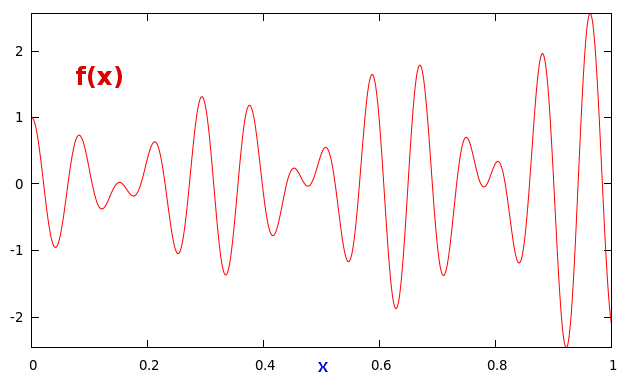
\includegraphics[scale=0.4]{f}
        \end{figure}
    }
    \only<2>{
        \begin{figure}[H]
            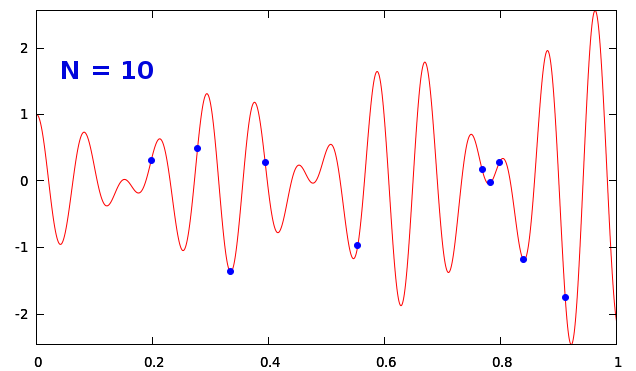
\includegraphics[scale=0.4]{f_10}
        \end{figure}
    }
    \only<3>{
        \begin{figure}[H]
            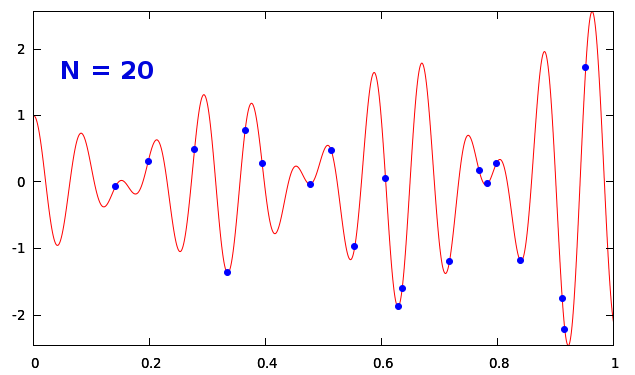
\includegraphics[scale=0.4]{f_20}
        \end{figure}
    }
    \only<4>{
        \begin{figure}[H]
            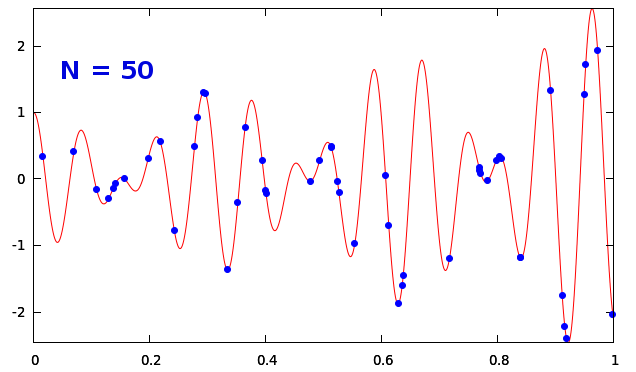
\includegraphics[scale=0.4]{f_50}
        \end{figure}
    }
    \only<5>{
        \begin{figure}[H]
            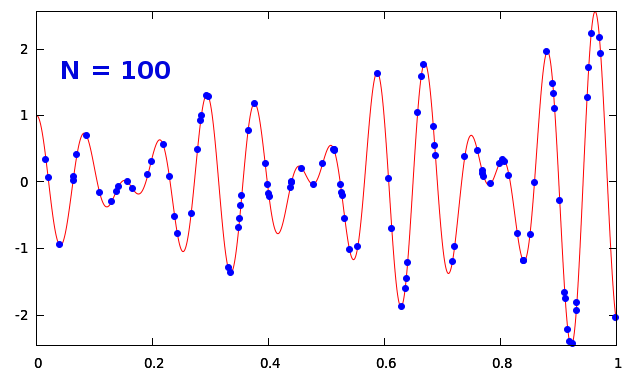
\includegraphics[scale=0.4]{f_100}
        \end{figure}
    }

\end{frame}

%\begin{frame}{References}
    %\raggedright
    %\nocite{*}
    %\bibliographystyle{plain}
    %\bibliography{master}
    %\vfill
    %\begin{center}
        %\Large
        %\textcolor{titlecolor}{\textbf{Any questions ?}}
    %\end{center} 
%\end{frame}

\end{document}
